% Fourier Analysis Introduction
In the beginning of the 1800s, Joseph Fourier was working on a physics problem called the heat equation, a certain partial differential equation. He had the idea of expressing the original function as a sum of sine and cosine functions as these would integrate and differentiate easily, making the differential equation easier to solve. He eventually developed and introduced the idea of Fourier series, a way of expressing a function as a sum of trigonometric functions \cite{Bounchaleun2019}.
% Fourier Series
\subsection{Fourier Series} 
If a function has a period of $2\pi$, the Fourier series takes the form $$f(t) = \frac{a_0}{2} + \sum_{n=1}^{\infty}a_ncos(nt)+\sum_{n=1}^{\infty}b_nsin(nt)$$ and states that a function can be represented by an infinite number of sine and cosine waves with different magnitudes and coefficients, plus some constant term. Using this representation and the properties of a few integrals of trigonometric functions, one can derive formulae for $a_0$, $a_n$ and $b_n$.

As an example, the following series $$\pi -2sin(x) -sin(2x) -\frac{2}{3}sin(3x) -\frac{1}{2}sin(4x) ... $$ is a sort of sawtooth wave. As a sawtooth wave is essentially just $f(x) = x$ over some interval it's relatively easy to compute the coefficients using the derived formulae. The same goes for the square and triangle waves, althought the triangle wave might be more difficult to calculate analytically.
 
% Fourier Transform
\subsection{Fourier Transform} 
The Fourier Transform is a operation that finds components that may be used to build a Fourier series. Formally it takes a function in time-domain (a signal as a function of time, like a sound) and outputs a function in frequency-domain, a kind of description for which kinds of sinusoids make up the original signal \cite{SimonXu2015}. Figure \ref{fig:transform} shows a signal and what it would look like in the frequency domain. If one added up the frequencies at the spikes in the frequency-domain (using the inverse of the Fourier transform), one would get back a very similar looking function to the original signal but without the noise. Unlike the Fourier series which works on periodic functions, the transform can be used to find the coefficients for non-periodic functions.

\begin{figure}[ht]
    \centering
    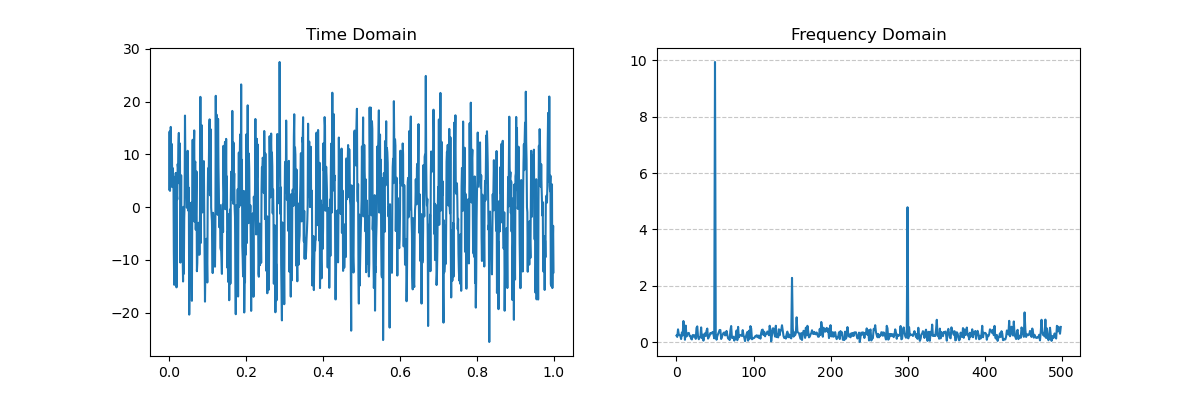
\includegraphics[width=\textwidth]{./images/transform.png}
    \caption{Some signal in the time-domain (displayed on the left) with added noise. Computing the transform with a discrete version of the Fourier transform reveals the main frequencies that make up the original signal in the time-domain (displayed on the right)\label{fig:transform}}
\end{figure}

Even though the the FT is an incredibly powerful function, its formula is compact. 
$$\hat{f}(\zeta) = \int_{-\infty}^{\infty} f(t)e^{-i2\pi\zeta t} dt$$
The variable $\zeta$ is used here to emphasize that the output is complex. It's also worth noting at this point that "transform" refers both to the act of transforming the function between domains but sometimes also the output values are called the transform.

% High level description of the Fourier transform.
\subsubsection{The big idea}
The idea behind the Fourier transform is that when some signal/function is multiplied by some sinusoid, if that sinusoid is a part of the signals, the frequencies "sync up" and if the sinusoid is not part of the signal, nothing special happens. On the interval $[0, 2\pi]$ any $sin(nx), n\in\mathbb{Z}$ will work against $sin(mx), m\in\mathbb{Z}$ and the "average" value is 0 except when $n=m$ in which case the "average" \todo{"average" is flaky}value is $\pi$. To get a non-zero "average" $n$ needs to equal $m$ which in turn implies that both signals contain a particular sinusoid. More formally 
\[ \int_0^{2\pi} sin(mx)sin(nx)dx = \int_0^{2\pi} cos(mx)cos(nx)dx= 
\begin{cases} % Some issues with cases
      0 & m\neq n \\
      \pi & m=n
   \end{cases} 
\]

% ---- Check the following statement with Antti: ----
The interval $[0, 2\pi]$ is only correct if $m, n \in \mathbb{Z}$. For the reals and rationals, the interval needs to be sufficiently large. The simplest way is to just integrate from $-\infty$ to $\infty$ like the formula wants us to and the respective integral will converge to either $0$ or $\pi$. Figure \ref{fig:transformIdea} shows how integer valued $m$ and $n$ work together or against eachother.

\begin{figure}[ht]
    \centering
    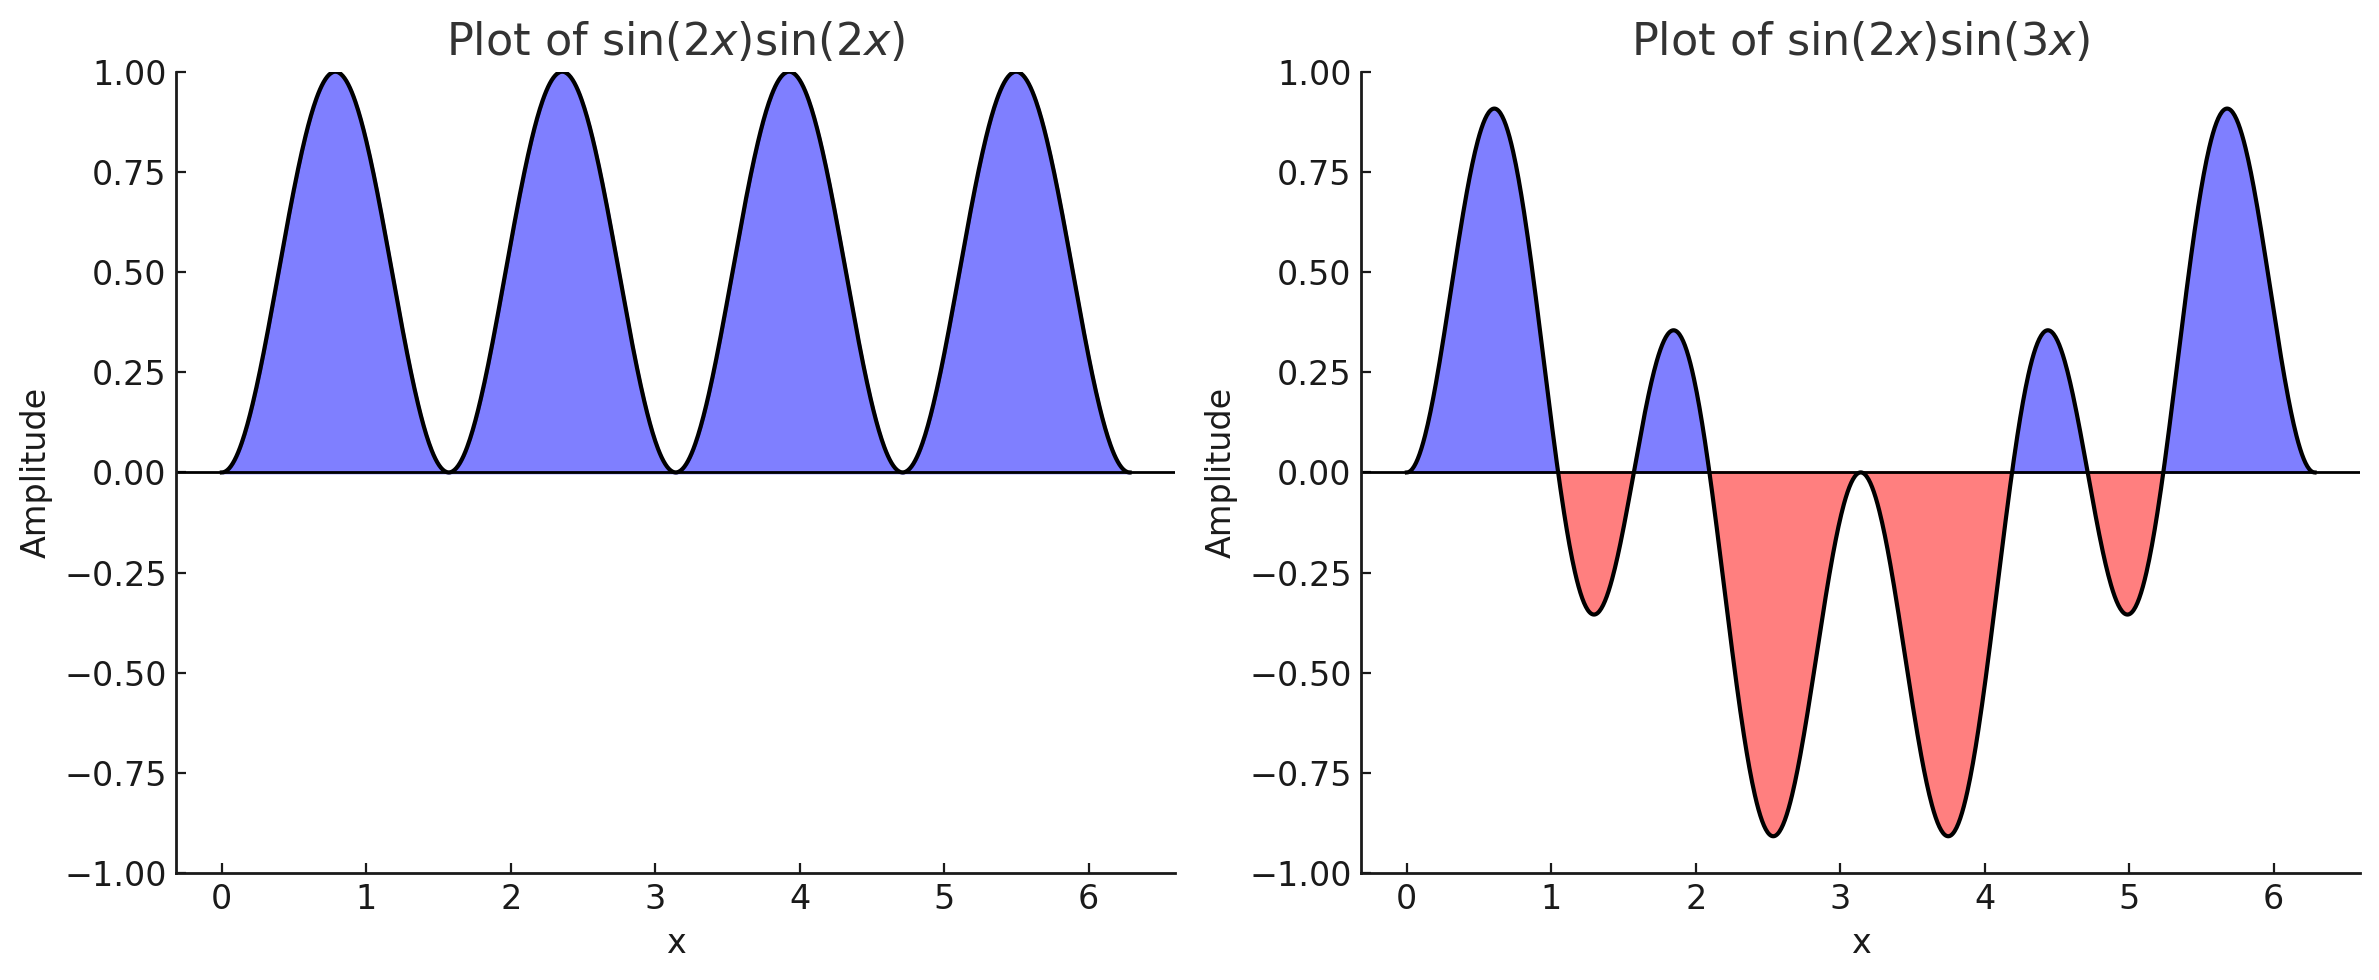
\includegraphics[width=\textwidth]{./images/transformIdea.png}
    \caption{The graphs of $sin(2x)sin(2x)$ and $sin(2x)sin(3x)$ on the $0$ to $2\pi$ interval. Matching $n$ and $m$ results in $sin^2(2x)$ which is always positive, resulting in a positive definite integral where as a mismatch causes equal positive and negative area, canceling out to 0.\label{fig:transformIdea}}
\end{figure}

% DFT
\subsection{Discrete fourier transform} 
The Discrete Fourier transform (abbreviated as DFT), as the name implies, is the Fourier transform for discrete signals. Instead of integrating over the entire function domain, we sum the samples from the signal starting from the start of the signal at $t=0$ to some $t=N$. The DFT for a signal $x$ with $N$ points is 
$$X_k = \sum_{n=0}^{N-1} x_ne^{-\frac{i2\pi kn}{N}}$$

% Matrix
\subsubsection{Matrix representation for the DFT computations} 
The DFT can be represented and computed by a matrix-vector multiplication. 
$$
% DFT coefficients
\begin{bmatrix}
    X(0) \\
    X(1) \\
    X(2) \\
    X(3) \\
    \vdots\\
    X(n) \\
\end{bmatrix}
=
% DFT matrix
\begin{bmatrix}
    1 & 1 & 1 & 1 & \cdots & 1\\
    1 & \omega & \omega ^2 & \omega ^3 & \cdots & \omega ^n\\
    1 & \omega ^2 & \omega ^4 & \omega ^6 & \cdots & \omega ^{2n}\\
    1 & \omega ^3 & \omega ^6 & \omega ^9 & \cdots & \omega ^{2n}\\
    \vdots & \vdots & \vdots & \vdots & \ddots & \vdots \\
    1 & \omega ^{n} & \omega ^{2n} & \omega ^{3n} & \cdots & \omega ^{{n^2}}\\
\end{bmatrix}
% Discrete signal
\begin{bmatrix}
    x(0) \\
    x(1) \\
    x(2) \\
    x(3) \\
    \vdots\\
    x(n) \\
\end{bmatrix}
$$
where $n = N-1$ as the computation are zero-indexed and $\omega$ is the principle N-th root of unity $e^{2\pi i/N} $. 

\todo{but why a matrix when the summation formula is both practical and more compact..? Also, FFT? What's the damn point?}

% Inverse transform
\subsection{Inverse Transforms}
The time-domain signal can be used, transmitted, received, but is hard to work with. The frequency-domain on the other hand is easy to work in, but makes little to no sense in many use cases. A C-major chord in frequency-domain can not be played, for example. The Fourier transform allows the transformation from time to frequency domain, but once any modification (like high frequency filtering) is applied, the signal needs to be transformed back to time-domain in order to be useful. The operation that does this is appropriately called the inverse Fourier transform, IFT for short or IDFT, for the discrete variant.

The inverse Fourier transform is very similar to the FT:
$$ f(t) = \frac{1}{\pi}\int_{-\infty}^{\infty} \hat{f}(\zeta)e^{i2\pi\zeta t} d\zeta$$
the discrete inverse transform (which should be called DIFT instead of IDFT) is 
$$ x_n = \frac{1}{N}\sum_{k=0}^{N-1} X(k)e^{\frac{i2\pi kn}{N}}$$.

% Computing
\subsection{Computations}
For pretty much any practical usage of the DFT, so many samples will be used that it's not feasible for to compute by hand. The DFT computations thus need to be converted to an algorithm or similar programmatic construct a computer can understand and run.
\subsubsection{Example DFT using the formula}
Even thought it's tedious, the formula is easy to use both in manual computations and when writing software for it. Given a discrete input signal $x = [-0.01298834,  0.62287525,  0.64266088,  0.39309558,  0.55407458, \cdots , -0.55613981, -0.55769558]$ which has a 100 elements, the DFT values can be computed with the formula $$X_k = \sum_{n=0}^{N-1} x_ne^{-\frac{i2\pi kn}{N}}$$. Starting with $k=0$ $X_0 \approx -0.3215+0i$, a number with both the real and imaginary components close to 0, which indicates very little impact on the original signal. At $k=5$ however, $X_k \approx 0.07725-24.5836i$ with a relatively large imaginary component. Repeating the same summation up to $k=100-1 = 99$ the other values of $X_k$ with relatively large imaginary components are at $k=12$ and $k=25$. 

To get the frequency-magnitude plot, the magnitudes for each $X_k$ are needed. The magnitude is the argument (length of the equivalent vector) of the DFT values and as a vector forms a right triangle, the length of the vector, or hypotenuse of the triangle can be computed with the Pythagorean theorem $a^2 + b^2 = c^2$. 

% Nyquist thing here

\subsubsection{Computing DFT with a programming language}
With the built-in complex data types and extensive mathematical and scientific computing libraries, implementing the DFT in Python is trivial. Leveraging Python's cmath library, the computations can be copied directly and 2 for-loops handles the summation and $X_k$ indexing as shown below.

\lstinputlisting[style=python]{../snippets/dft.py}

For a more primitive language like C, without complex exponentiation, the computations are still fairly straightforward to do due to Euler's formula that expands $e^{ix} = cos(x) + isin(x)$. The components can be separated into two separate data structures and so the imaginary unit can be dropped. A possible C implementation (without using a struct for complex numbers) is shown below. 

\lstinputlisting[style=c]{../snippets/dft.c}

These examples are purely illustrative, there's no reason to implement the DFT in practice because there are algorithms that do the same transformation, just with less computations, and the difference just grows with the sample size.
\subsubsection{Computing the inverse}
Writing the inverse discrete Fourier transform in Python is as straightforward as the DFT due to the cmath library, but an additional normalization is added as shown below 


\lstinputlisting[style=python]{../snippets/idft.py}

The signal that we are turning back to the time-domain is filtered very naively for demonstration purposes. The filter turns unimportant frequencies (components with a magnitude less than 2) to 0. Figure \ref{fig:DFT-IDFT} shows both the original signal and filtered signal in both time and frequency-domain.

\begin{figure}[ht]
    \centering
    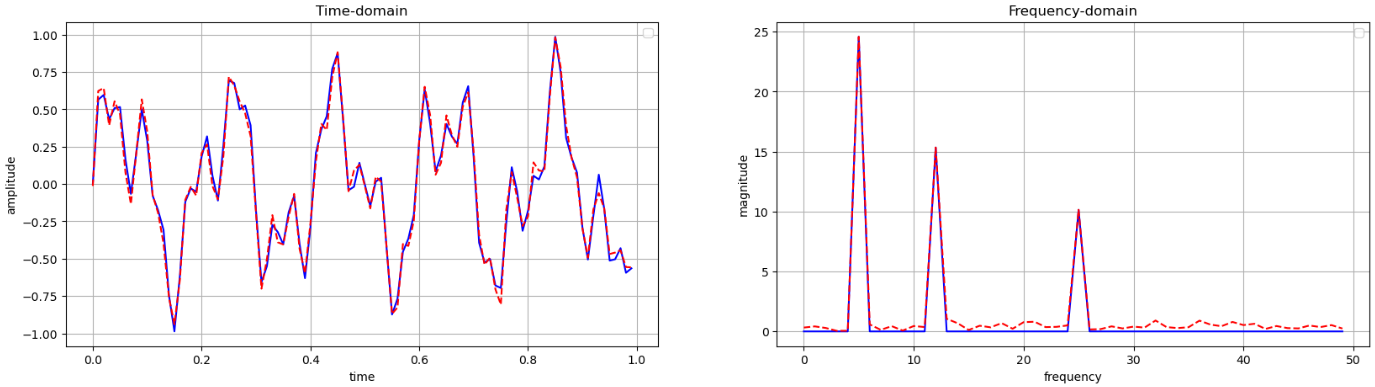
\includegraphics[width=\textwidth]{./images/filtered_signal.png}
    \caption{The time-domain and frequency-domain representations of the signal (red dashed line) and the filtered signal (blue solid line). When on top of eachother, one can observe more regularity in the blue graph in the time-domain.\label{fig:DFT-IDFT}}
\end{figure}

% FFT
\subsection{Fast fourier transform}
The DFT takes $n^2$ operations to perform as there are $n$ outputs $X_k$ and $n$ amount of numbers are summed. A fast fourier transform (abbreviated as FFT) is any method that speeds up the computation of the DFT. This means that even if there is one Fourier transform and basically one DFT, there are multiple FFT algorithms. One could argue, however, that very few users of the FFT cares about the underlying algorithm, they just expect the functionality of the DFT, but faster. 

\subsubsection{Time complexity}
Time complexity refers to the asymptotic performance of an algorithm. Even though it in many cases correlates with real performance, it's ultimately theoretical and only considers the highest order term, because it's the biggest contributor when the input size grows towards infinity. For example, consider an algorithm for multiplying 2 numbers. One such algorithm is taught in elementary school and multiplies every digit with every other digit, shifting one step for every iterations for multiplying by a power of 10 then adding all numbers together to get the final result. This algorithm takes $N^2+N$ steps but as N grows larger and larger, the $N^2$ term will contribute the most, so we say that the algorithm has a complexity of $O(N^2)$, called Big-O. For multiplying two 1000 digit long integers, the multiplication will take a million operations and the summation will take 1000. Increasing the input size with 1 digit adds only 1 more addition, but it adds 1001 more multiplication steps.

Perhaps the most popular algorithms, the Cooley-Tukey FFT, has an algorithmic complexity of $O(n \log n)$, a significant speed up over $O(n^2)$ \cite{Randhawa2018} \cite{HeidemanEtAl1984}. Once in Big-O, the base of the logarithm does not matter, the only thing that matters is that it is logarithmic \todo{Does this need source?}. An improvement from $O(n^2)$ to $O(n \log n)$ means that even with a mere 1000 samples, the speed up, purely in terms of time complexity, is around 100x. In a paper by James Cooley, he examplified a computation with the Fourier transform of a dataset of 512000 data points which he claims would see an around 12800x speedup with the FFT \cite{Cooley1987}. 512000 data points would take on the order of 262 billion operations to complete with an $O(n^2)$ algorithm, which with a modern personal computer can take minutes to complete. An $O(n \log n)$ algorithm takes a relatively measly 9.7 million operations and runs in milliseconds. This is akin to measuring the execution time of Quick sort to Bubble sort for an array of size 512000 which indeed sees around a 12800x speedup.

This speedup in execution time and theoretical time complexity improvement demonstrates the power of the FFT. Why this improvement is so important will hopefully be evident after the chapter on the applications of Fourier methods, but essentially, the FFT is considered by some  to be one of the most important algorithms in history due to being able to perform important (every-day) heavy computations instantenously. 

\subsubsection{Brief history of the FFT} \todo{this whole section is bad, I'll either fix it or remove it later}
The history of the FFT is long and cloudy with multiple scientists working on a similar problem between 1800-2000. Cooley and Tukey introduced their algorithm in 1965 and at the time it was regarded as a completely new and revolutionizing algorithm. Based on the papers [A] and [B], the FFT and similar numerical methods were developed in two chains. One of them was started with Euler and Lagrange which Gauss based his work on. Runge's work is based on ????????? Gauss and was the basis for a lot of other development. The other chain, which seemingly does not link to Gauss is where Cooley-Tukey exists. They tributed I.J. Good in their paper even though their algorithm was pretty different from the Good one, which is now commonly called the Prime Factor Algorithm and sometimes Good-Thomas. 

% Yates used? FFT for a convolution

It was later discovered that Cooley-Tukey works almost exactly as the algorithm Gauss had proposed almost a century earlier. This is probably why Cooley talks about the "re-discovery" in one of his paper. Since the algorithm was only rediscoverd by Cooley and Tukey, some would like to give Gauss more credit for the FFT and some authors have used terms such as "Discrete Gauss Transform (DGT)" and "Gauss-Fourier Transform (GFT)". To make the history of the FFT even muddier, Clairaut published a cosine-only "DFT" 50 years before Fourier even came forth with the Fourier series. Lagrange came up a sine-only DFT-like formula around 40 years before Fourier series.

% At first, the Cooley-Tukey algorithm was regarded as an entirely new thing.   
% The modern FFT (what's that?) is based on the work of Gauss, almost which was developed almost a century before Cooley-Tukey. Gauss and CT use the same algorithm but the equivalence is not obvious due to Gauss' obscure and outdated notation.

% Some would like to credit Gauss with the FFT even though it would be impractical. Some have and there have been uses of the terms "Discrete Gauss transform (DGT)" and " Gauss-Fourier transform (GFT)".

% In the 1800s, an FFT which was NOT based on Gauss was widely used

% Clairaut published a cosine-only "DFT" in 1754, 50 years BEFORE Fourier's Fourier series??? Lagrange came with a sine-only DFT-like formula in 1762


% CT > Good > Thomas, Yates
% Rudnick > Danielson-Lanczos > Runge 
% Gauss > Lagrange, Euler
% Smith > Darwin > Thompson > Runge
% Smith > Everett > Darwin & Smith > Kelvin > Everett > Darwin
% What is the link between Thomas, Yates and the "rest"?
% What's the link between Gauss and Runge
% Where does Carlini fit into the picture?

\subsubsection{FFT Algorithm}
As previously mentioned, FFT is simply put any algorithm that computes the DFT fast. One of the easier to understand but still demonstrates the workings of the algorithm is the Radix-2 FFT. The Radix-2 FFT is easy to understand because it assumes the input size is a power of 2, meaning it's easy to recursively split in two. On a high level, the Radix-2 algorithm starts with splitting the input array into odds and evens. It then calls itself for the odds and evens, recursively splitting the array. On the way back, it performs the DFT on smaller units of the original signal, utilizing the symmetry of roots of unity to perform multiple operations at once. \todo{this could be reworked?}

To derive the Radix-2 FFT, the DFT is split into two sums, one for the even indeces and one for the odd $$X_k = \sum^{N/2-1}_{n=0} x_{2n}T^{2n}+ \sum^{N/2-1}_{n=0} x_{2n+1}T^{2n+1}$$, where $T$ is the so called twiddle factor $e^{-\frac{2\pi ik}{N}}$. A common twiddle factor is factored out of the odd sum and the even and odd sums are denoted as $E_k$ and $O_k$ respectively. 

$$X_k = E_k + TO_k$$

These functions $E_k$ and $O_k$ are periodic with a period $N/2$ which can be shown by showing that $$e^{\frac{-2\pi in(k+N/2)}{N/2}} = e^{\frac{-2\pi in(k)}{N/2}}$$
which means that 
$$E_k = E_{k+\frac{N}{2}}, O_k = O_{k+\frac{N}{2}}$$
Since this holds true for $E_k$ and $O_k$, the following is also true

\[
X_k = \left\{\begin{array}{lr}
    E_k + TO_k, & \text{for } 0 \leq k < N/2\\
    E_{k-N/2} + TO_{k-N/2}, & \text{for } N/2\leq k< N\\
    \end{array}\right\}
\]
this is saying that the DFT can be computed in two layers, the lower $N/2$ terms and the upper $N/2$ terms.
When computing the upper $N/2$ terms, i.e. when $N/2 \leq k < N$, $X_k = E_{k-N/2} + T^{N/2}O_{k-N/2}$, which are the same O and E as the lower $N/2$ terms, just with an offset of N/2. The twiddle factor is raised to the power of N/2 because it too is in terms of k. We can thus split $X_k$ into \todo{This section could be reworked}

$$X_k = E_k + TO_k$$  
$$X_{k+N/2} = E_k + T^{N/2}O_k$$
which are the equations for the lower and upper $N/2$ terms. Finally the twiddle factor is rewritten using the following property of complex exponentials

$$e^{\frac{-2\pi i(k+N/2)}{N}} = -e^{\frac{-2\pi i(k)}{N}}$$
which gives

$$X_k = E_k + TO_k$$  
$$X_{k+N/2} = E_k - TO_k$$

Recall that

$$E_k = \sum^{N/2-1}_{n=0} x_{2n}T^{2n}$$
$$O_k = \sum^{N/2-1}_{n=0} x_{2n+1}T^{2n}$$
and that the DFT is
$$X_k = \sum^{N}_{n=0} x_nT^{n}$$
This means that when the element indeces are adjusted, $E_k$ and $O_k$ are both DFTs essentially. To transform (no pun intended) \todo{can I keep this?} this purely mathematical notation into something that looks more like a complete algorithm, express the computations with a loop

\begin{lstlisting}
do k = 0, N/2-1
    T = exp(-2*i * PI * k / N) 
    X(k+1) = E(k+1) + T * O(k+1)
    X(k+1 + N/2) = E(k+1) - T * O(k+1)
end do
\end{lstlisting}
In Fortran, arrays are indexed starting from 1, this means that every array access needs an offset of 1. Before these computations we need to compute the evens and odds.
\begin{lstlisting}
E = r2fft(input(1:N:2))
O = r2fft(input(2:N:2))
\end{lstlisting}
Any recursive algorithm also needs a base case.
\begin{lstlisting}    
if (N == 1) then
    X = input
    return
end if
\end{lstlisting}
Putting everything together and adding variable declarations and initialization as well as the function declaration, a naive Radix-2 FFT could look like the following

\lstinputlisting[style=fortran]{../snippets/fft.f90}

% Source of proof: https://www.phys.uconn.edu/~rozman/Courses/m3511_19s/downloads/radix2fft.pdf

This algorithm assumes the input is a power of 2 but the implementation does not handle it anywhere. The program still runs, but to no surprise gives an erroneous answer. Figure \ref{fig:FFT-Alg} shows a block diagram of the FFT computations.

\begin{figure}[ht]
    \centering
    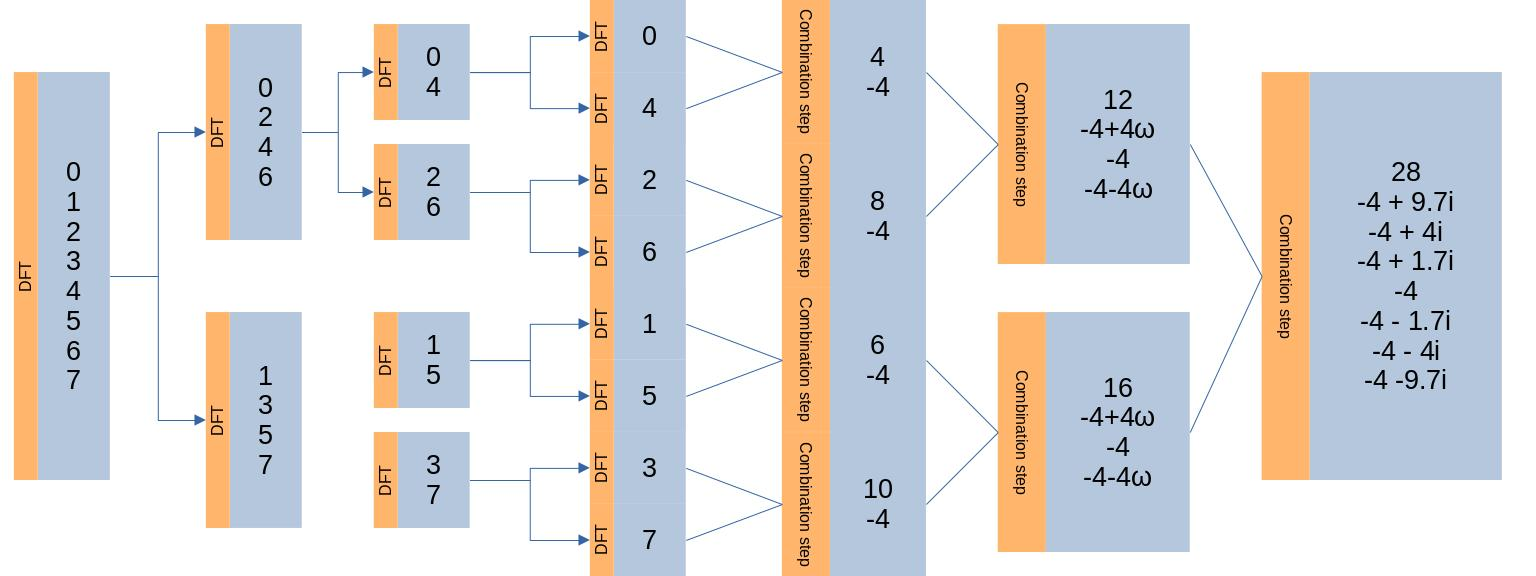
\includegraphics[width=\textwidth]{./images/fft.jpg}
    \caption{Diagram of an FFT with 8 elements. The process starts with splitting down the input vector to the recursive base case $N=1$. After that the values are combined using the core computations of the Radix-2 FFT. The right-most column in the graph is the output transform of the left-most column.\label{fig:FFT-Alg}}
\end{figure}

\subsubsection{Inverse FFT}
The inverse of the FFT can be derived using the DFT matrix previously shown. It can be shown that inverting the DFT matrix results in a very similar matrix, but with all exponents of the twiddle factor negated and with a normalization scaling. In \cite{Reducible2020} it is shown that the IFFT algorithm can reuse the FFT logic, with a single line changed. At the time of writing, popular Python library Numpy utilizes the same \_raw\_fft method to compute both FFT and IFFT. \todo{does this need source?} 

%https://github.com/numpy/numpy/blob/main/numpy/fft/_pocketfft.py
\subsubsection{Notable FFT implementations}
\textbf{Fastest Fourier Transform in the west}, more known by it's acronym FFTW, is a ...
\textbf{PocketFFT}, used by Numpy






